\section{Novos \textit{datasets} para a língua de sinais}
\label{sec:metodologia-datasets}

Conforme introduzimos acima, o primeiro passo para que possamos desenvolver e avaliar uma abordagem de aprendizagem de máquina centrada na linguística da língua de sinais consiste em definir um conjunto de dados que viabilize isso. Como a proposta apresentada aqui é nova e, devido a isso, não há \textit{datasets} diretamente compatíveis com ela, optamos por derivar um novo \textit{dataset} a partir de outro já existente -- o \acrfull{asllvd}.

O \acrshort{asllvd} consiste em um amplo \textit{dataset} público\footnote{Disponível em \url{http://www.bu.edu/asllrp/av/dai-asllvd.html}} da \acrshort{asl} que contém aproximadamente 2.745 sinais representados em cerca de 9.763 sequências de vídeo articuladas por indivíduos Surdos nativos. Suas amostras são capturadas por meio de quatro câmeras sincronizadas: uma visão frontal de alta resolução a meia velocidade, outra visão frontal de resolução total, uma visão lateral e uma visão da face, conforme ilustrado na \autoref{fig:asllvd-example}~\cite{athitsos-2008-asllvd,neidle-2012-asllvd}.

\begin{figure}[ht!]
    \centering
    \caption{\textmd{Exemplo de três perspectivas sincronizadas providas pelo \acrshort{asllvd} para o sinal MERRY-GO-ROUND: 
    frontal (\subref{subfig:asllvd-example-front}), 
    lateral (\subref{subfig:asllvd-example-side}) e 
    face (\subref{subfig:asllvd-example-close}).}}
    \subcaptionbox{\label{subfig:asllvd-example-front}}{
        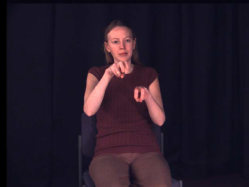
\includegraphics[width=0.25\textwidth]{imagens/metodologia/datasets/asllvd_example_front}
    }%
    % \hfill
    \subcaptionbox{\label{subfig:asllvd-example-side}}{
        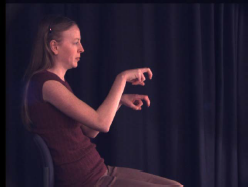
\includegraphics[width=0.25\textwidth]{imagens/metodologia/datasets/asllvd_example_side}
    }%
    % \hfill
    \subcaptionbox{\label{subfig:asllvd-example-close}}{
        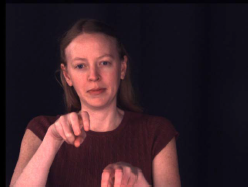
\includegraphics[width=0.25\textwidth]{imagens/metodologia/datasets/asllvd_example_close}
    }%
    \nomefonte[p. 2]{athitsos-2008-asllvd}
    \label{fig:asllvd-example}
\end{figure}


Para que fosse possível computar parâmetros fonológicos a partir dos frames das amostras do \acrshort{asllvd}, que consistem em imagens RGB bidimensionais, realizamos um processo de duas etapas:

\begin{enumerate}
    \item A partir da combinação de diferentes perspectivas dos sinalizadores, estimamos as coordenadas dos esqueletos dos indivíduos no espaço 3D, frame-a-frame. Essa etapa originou um \textit{dataset} intermediário chamado ASL-Skeleton3D, que pode ser utilizado por outras pesquisas para derivar novas representações.
    \item Com base nesses esqueletos 3D, finalmente calculamos os parâmetros fonológicos dando origem ao \textit{dataset} final ASL-Phono.
\end{enumerate}


Esse processo trouxe consigo alguns desafios computacionais, entre os quais podemos enumerar:

\begin{enumerate}
    \item Definição de uma abordagem para reconstruir o espaço 3D a partir das frames de vídeo simples em 2D do \acrshort{asllvd}, bem como para lidar com amostras ausentes ou de baixa qualidade encontradas.

    \item Definição de um conjunto inicial de atributos fonológicos que pudessem capturar e representar variações significativas do corpo durante a articulação dos sinais e que também pudessem ser representados computacionalmente.
    
    \item Identificação de abordagens matemáticas e antropométricas que permitissem o cálculo e a representação desses atributos.
    
    \item Processamento de mais de 9.000 amostras para cada um dos \textit{datasets}, que consumiu recursos computacionais caros, como 40 horas contínuas de processamento distribuído com CPU e GPU, e mais de 1 TB de dados gerados.
\end{enumerate}



\subsection{ASL-Skeleton3D}
\label{sec:metodologia-datasets-3d}




% \subsection{ASL-Phono}
% \label{sec:metodologia-datasets-phono}